\section{Metode og proces}

For at sikre en effektiv udviklingsproces, har vi valgt at anvende en agil udviklingsmetode, specifikt Scrum.
Valget er foretaget på baggrund af en metodisk analyse af projektets rammebetingelser.

\subsection{Analyse af projektets karakteristika}
Ved hjælp af Boehm og Turners radar-diagram er projektet blevet vurderet ud fra fem dimensioner: Personnel, Physical Size, Criticality, Culture og Dynamism.~(\cite{BoehmTurner})
Analysen har tjent til at tage en informeret beslutning om hvilken grad af agil tilgang er mest hensigtsmæssig. Herunder skrildres et udfyldt radar-diagram samt en kort opsummering af overvejelser for projektet i relation til de fem dimensioner:

\begin{figure}[h]
    \centering
    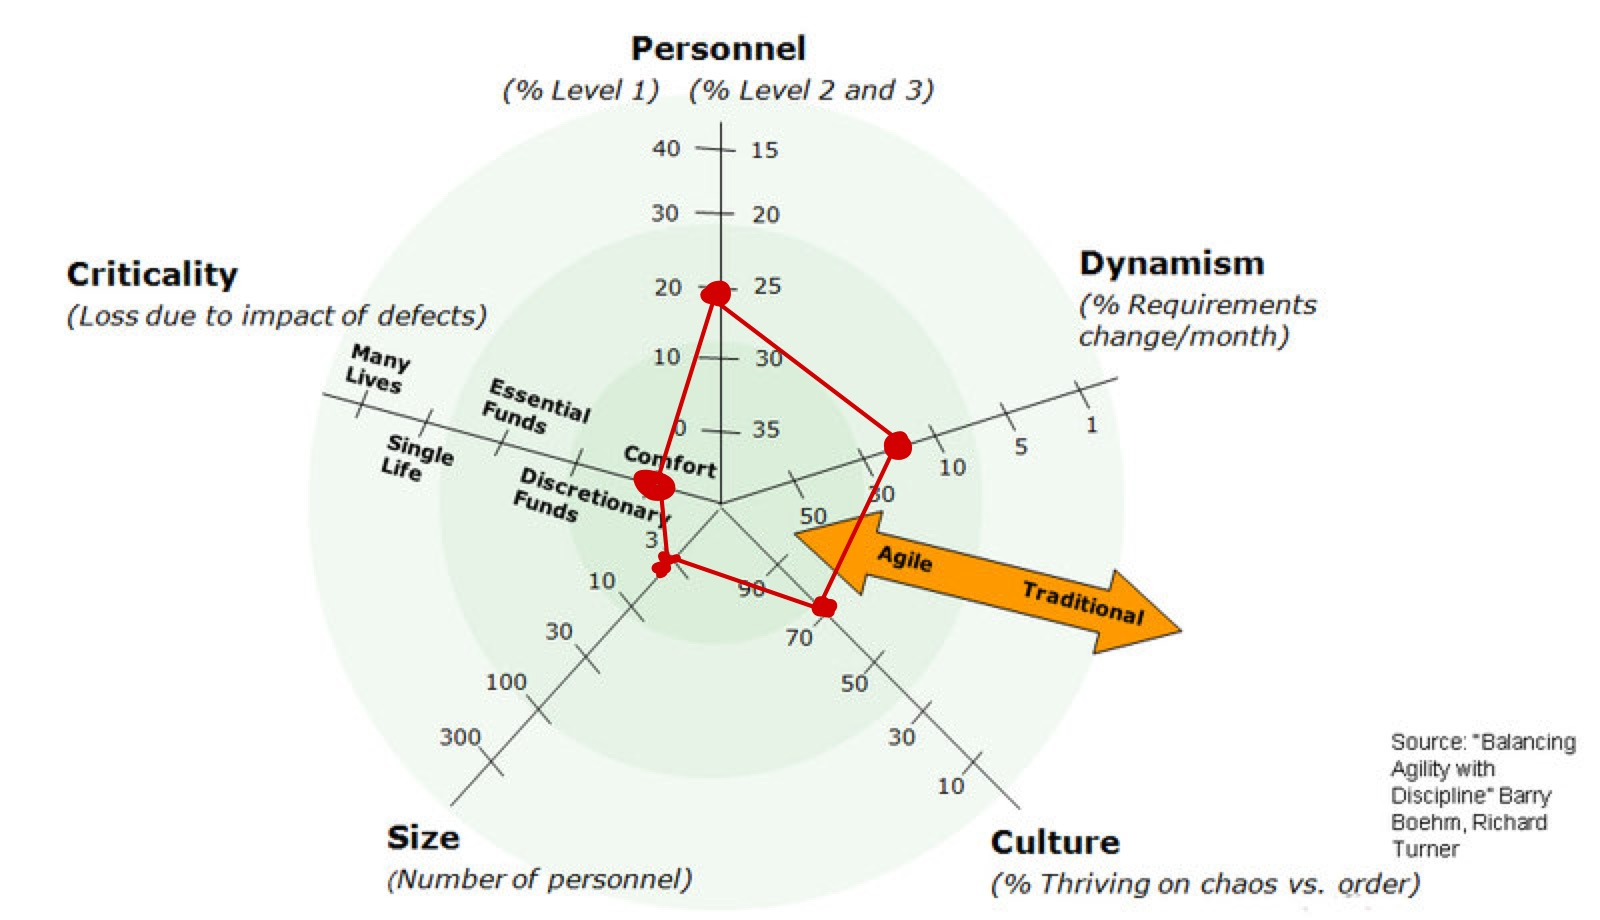
\includegraphics[width=0.8\textwidth]{Dokumenter/bilag/Diagrammer/Boehm-Turner-Radar-Diagram.pdf}
    \caption{Boehm og Turners radar-diagram for projektet}
    \label{fig:boehm-turner-radar}
\end{figure}

Ud fra analysen, som blev udført i projektets indledende fase, blev det fastlagt, at projektet har de følgende karakteristika:
\begin{itemize}
    \item Meget lille teamstørrelse som en bachelorgruppe på 3 (Size)
    \item et lavt til moderat niveau af expertise, fordi vi er næsten færdiguddannede bachelorstuderende, men heller ikke senior developers (Personnel)
    \item lav kritikalitet, da de klarer sig nogenlunde med eksisterende løsninger og deres forening ikke står og falder med produktet. (Criticality)
    \item en kultur, der er åben for forandring og innovation (eller `kaos'), da vi er i en læringsfase og ønsker at eksperimentere med nye teknologier og metoder (Culture)
    \item en høj grad af usikkerhed og foranderlighed i kravene, da vi forventer at skulle tilpasse og ændre vores tilgang baseret på feedback og læring undervejs (Dynamism)
\end{itemize}

Som det tydeligt fremgår af diagrammets centrum-nære punkter, læner projektet sig mod en agil tilgang.

\subsection{Beskrivelse af udviklingsmetode}

Analysen har ført til udarbejdning af en procesmodel med skærpet fokus på dokumentation til både underviser/censor i form af en rapport og interessent.

\subsubsection{Agilt værktøj}
Processen udføres som Scrum-inspirerede sprints af to ugers varighed, understøttet af projektstyringsværktøjet Taiga~(\cite{Taiga}).
Taiga er blevet valgt for sin enkelthed og fordi programmet er FOSS, hvilket passer godt til vores projekt og værdier. Gruppen havde intention om at hoste programmet selv for læring, men endte med at bruge Taigas cloud-løsning, da deres free plan opfyldte vores behov og krævede minimal opsætning.
For at sikre sammenhæng mellem de overordnede mål og gruppens daglige eksekvering, er alle User Stories i projektets backlog blevet mappet til specifikke krav i kravspecifikationen. Denne sporbarhed støtter, at udvikligen altid bidrager til opfyldelsen af de definerede systemkrav.

\subsubsection{Daglig Koordination og Sprintplanlægning}
Teamet deltager ved hvert arbejdsmøde i en 5 minutters stand-up, der dækker hvad man har gjort siden sidste møde og hvad man vil gøre inden næste.
I forbindelse med sprint-skifte holdes et udvidet møde, hvor teamet evaluerer det forgangne sprint og planlægger det næste. 
Hvert sprint indledes med en planlægningssession, hvor teamet udvælger User Stories fra backloggen, der skal arbejdes på i det kommende sprint.


\subsubsection{Itemization}
Umiddelbart efter sprintplanlægningen, gennemføres itemization af de valgte User Stories.
En central del af processtrategien er håndteringen af teknisk usikkerhed gennem en `Just-in-Time' tilgang til detaljeplanlægning:
Ved sprintstart udvælges de højest prioriterede User Stories fra backloggen. Først når en User Story trækkes ind i et aktivt sprint, foretages en detaljeret itemization.
Rationalet er, at vi - baseret på overvejelser efter samtale med vejleder - minimerer spildt planlægningsarbejde på krav, der potentielt ændrer sig, og sikrer, at den tekniske nedbrydning baseres på den nyeste viden i teamet.

\subsubsection{Definition af Done og Test}
Kvalitetssikringen er integreret direkte i sprint-cyklussen. 
En User Story anses først for færdig, når samtlige tilknyttede items er implementeret, og der er gennemført en dedikeret testfase på User Story-niveau.
For at vedligeholde agiliteten er er ikke krav til at user stories skal være programmatisk testet (unit/integration), men der indgår review og testing i vores github workflow, hvor en pull request først can merges, når den er blevet reviewet og godkendt af mindst én anden person i teamet.
Dette sikrer, at funktionaliteten ikke blot er teknisk implementeret, men også verificeret mod de acceptkriterier, der er defineret i kravspecifikationen, at at dette verificeres af et andet medlem af teamet end den udvikler, der har implementeret den.

\subsection{Procesforløb og retrospektiv (?)}
